\documentclass[border=8pt]{standalone}
\usepackage{fontspec}
\setsansfont{Arial}
\usepackage{pgfplots}
\pgfplotsset{compat=1.18,
  every axis/.append style={/pgf/number format/assume math mode=true,
    tick label style={font=\sffamily\small}}}
% Case recall of a k-of-4 rule when the four components are found independently with
% equal recall r (binomial model, Equation in Section 3.7). Analytical, not measured.
\begin{document}
\sffamily\small
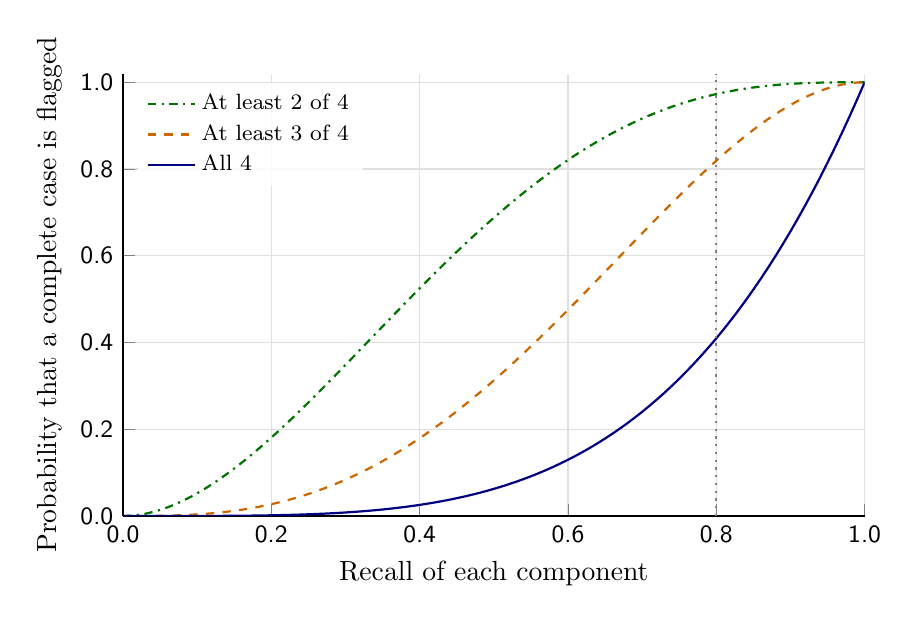
\begin{tikzpicture}
\begin{axis}[
  width=11cm,height=7.2cm,xmin=0,xmax=1,ymin=0,ymax=1.02,
  xlabel={Recall of each component},ylabel={Probability that a complete case is flagged},
  xtick={0,0.2,...,1.0},ytick={0,0.2,...,1.0},
  xticklabel style={/pgf/number format/.cd,fixed,fixed zerofill,precision=1},
  yticklabel style={/pgf/number format/.cd,fixed,fixed zerofill,precision=1},
  grid=major,grid style={black!12},axis lines*=left,
  domain=0:1,samples=101,
  legend style={font=\footnotesize,draw=none,fill=white,fill opacity=0.85,text opacity=1,at={(0.02,0.98)},anchor=north west},
  legend cell align=left]
\addplot[green!45!black,thick,dashdotted] {1-(1-x)^4-4*x*(1-x)^3};
\addplot[orange!80!black,thick,dashed] {4*x^3*(1-x)+x^4};
\addplot[blue!50!black,thick] {x^4};
\legend{{At least 2 of 4},{At least 3 of 4},{All 4}}
\draw[black!50,dotted,thick] (axis cs:0.8,0)--(axis cs:0.8,1.02);
\end{axis}
\end{tikzpicture}
\end{document}
